\chapter{Successional shifts in the root-associated microbiota throughout the life cycle of the crop plant \textit{Oryza sativa}}

Joseph Edwards\footnote[1]{Department of Plant Biology, University of California, Davis}, Christian Santos$^1$, Zach Liechty$^1$, Bao Nguyen$^1$, Nicole Chan$^1$, Eugene Lurie$^1$, and Venkatesan Sundaresan$^1$

\section{Abstract}
Much like how humans host a gut microbiota, plants assemble a root-associated microbiota which can aid the plant in assimilating nutrients, reducing susceptibility to pathogens, and alleviating the severity of abiotic stresses. Plants host microbiota in at least 3 distinct root-associated compartments: the rhizosphere, rhizoplane, and endosphere. It is unclear how the communities in these compartments shift over the course of the plant's life cycle or whether the transition to the reproductive phase has any effect on the root-associated microbiota. Here, we characterize the root-associated microbiota of the cereal crop \textit{Oryza sativa} over the course of 3 seasons. We found that the microbiota in each root-associated compartment shifts significantly over the life cycle of the plant and that these shifts are independent from the shifts in unplanted soil and are consistent from season to season. We found that the root microbiota shifts rapidly until the entry into the reproductive phase, whereupon the microbiota stabilizes. Using a machine learning framework, we identified taxa that were discriminant of plant age. We next investigated whether there exists a developmental stage-specific microbiota by sampling rice varieties with different developmental progression rates. Again using a machine learning approach, we were able to identify bacterial taxa whose abundance patterns are discriminant of plant developmental stage. These results indicate that changes in plant development either directly or indirectly impact the root-associated microbiota.

\section{Introduction}
Plants derive root-associated microbial communities from the soil which are inhabited by thousands of different species and strains of archaea and bacteria \cite{Lundberg2012,Bulgarelli2012,Peiffer2013,Edwards2015,Wagner2016}. Individual taxa within the root-associated microbiota have been found to be beneficial for plant growth and resistance to biotic and abiotic stresses \cite{Bulgarelli2013,Berendsen2012,Mendes2011}. In rice, we previously identified three spatially distinct root compartments with significantly different microbiota compositions: the soil adjacent to the root (the rhizosphere), the root surf,ace (the rhizoplane), and the root interior (the endosphere) \cite{Edwards2015}. It was found that each of these root-associated compartments have significantly different microbiota profiles from the communities in unplanted soil, thus indicating the roots enrich for subsets of the soil microbiota. This enrichment process and how the root-associated microbiota shift throughout the lifecycle of rice plants remain uncharacterized.

In humans, the successional shifts in the gut microbiota have been well studied from infancy into adulthood \cite{Koenig2011,Mueller2015,Backhed2015,Yatsunenko2012}. Newborns are characterized by a low diversity gut microbiota that increases with age \cite{Koenig2011}. The composition of the human gut microbiota shifts rapidly during the first three years of life, then stabilizes to become more like an adult microbiota after three years and these shifts correlate well with dietary intake \cite{Yatsunenko2012}. Whether a similar developmental  trend occurs within the root-associated microbiota of plants remains unclear. In this study, we detail the succession of microbial consortia in the three root-associated compartments of rice while being cultivated under field conditions. We also characterize how plant developmental progression is associated with the succession of various taxa.

\section{Results}
\subsection{Experimental Design and Sequencing}
We first were interested in monitoring how root-associated microbiotas shift throughout the life cycle of the rice plant under field conditions and whether changes in community profiles were consistent across multiple seasons. To do this, we collected the rhizosphere, rhizoplane, and endosphere microbiota samples from rice plants grown in a submerged commercial rice field in Arbuckle, California over the 2014 and 2015 seasons. In 2014, the field was sampled weekly until harvest, a total of 19 weeks with each time point consisting of 8 replicates. In 2015, because we were interested in the initial root colonization stage, we sampled every other day for the first 4 weeks of growth, thereafter sampling every other week until harvest. Each time point in 2015 consisted of 4 replicates. For each season, we collected bulk soil (i.e. soil from the submerged field where no roots were growing) until root growth made it impossible to locate soil unaffected by rice roots: around 4 weeks for the 2014 season and 6 weeks for the 2015 season.

PCR amplification and Illumina sequencing of the 16S rRNA gene was conducted to profile microbial communities present in each sample. Operational Taxonomic Unit (OTU) clustering was done at the 97\% threshold using the NINJA-OPS pipeline \cite{Al-Ghalith2016}. We detected a total of 24,048 OTUs across 1,290 samples with a total of 48,954,921 sequences. We removed a total of 276 detected OTUs matching mitochondrial or plastidial taxonomies. We then removed samples from our dataset with less than 1000 total reads. One difficulty of microbiome studies is to perform statistics on non-reproducible OTUs. We removed OTUs from our dataset that were not present in at least 5\% of the total samples. This step reduced our dataset to 8,554 OTUs for analysis.

\subsection{Microbiomes are shaped by distance from the root and plant age}
\begin{figure}[h]
\centering
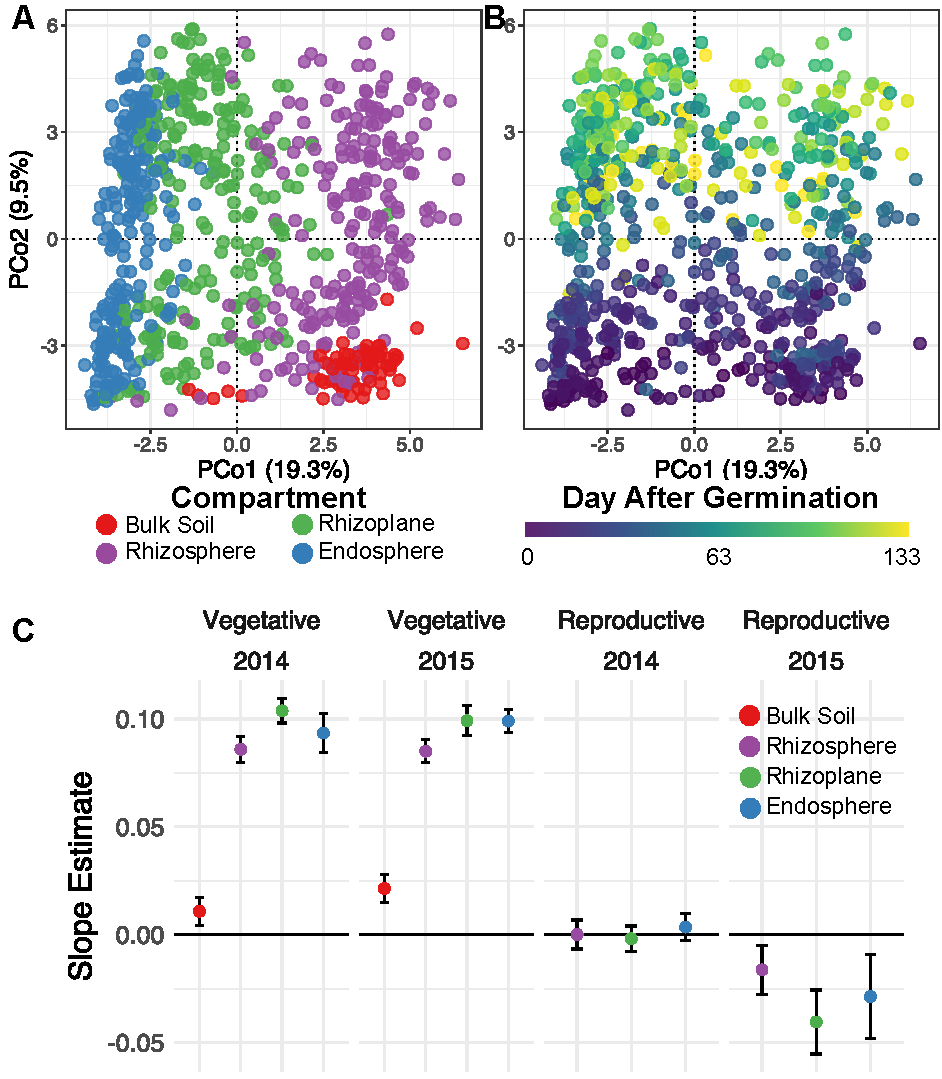
\includegraphics[width=5in]{Figures/figure3_1}
\caption[Figure 4.1]{\textbf{The root-associated microbiota is differentiable by root compartment and plant age.} \textbf{(A)} Principal coordinate analysis (PCoA) of Bray-Curtis distances between samples colored by root-compartment. \textbf{(B)} The same plot as in A but colored by the age of the plant from which the samples were obtained. \textbf{(C)} The estimated slope of the second prinicipal coordinate of plot A as a function of plant age. We fit separate linear models to estimate that slope during the vegetative phase and the reproductive phase (defined as plants older than 63 days) for each compartment. The 2014 and 2015 seasons' data is included in plots A and B.}
\label{Figure 4.1}
\end{figure}

To understand the underlying driving forces of microbial community variation in our data, we used Principal Coordinates Analysis (PCoA) of Bray-Curtis distances. We found that samples from 2014 and 2015 display a spatial pattern of divergence along the first principal coordinate, where communities in bulk soil samples cluster on one end of the axis and endosphere communities cluster on the other (Fig. 4.1A). In agreement with our previous studies on the rice root-associated microbiomes \cite{Edwards2015}, perMANOVA of pairwise distances between samples indicated that microbial communities differed significantly between root-associated compartments (R2 = 0.23, P = 0.001). 

We next measured the effect of plant age on the root-associated microbiota. PerMANOVA of pairwise distances between samples revealed that plant age had a significant effect on the root-associated microbiota (R2 = 0.21, P = 0.001). We found that this effect was captured on the second principal coordinate of the PCoA plot (Fig. 4.1B). In the M206 cultivar, panicle initiation (entry into reproduction) occurs 56-63 days after germination \cite{Linquist2012}. We quantified the slope of the second principal coordinate in response to plant age for the vegetative stage (days < 63) and the reproductive stage (days >= 63) using a linear model. We found that in each root-associated compartment, the rate of change (i.e. the linear slope estimate) was reduced in the reproductive phase compared to the vegetative phase (Fig. 4.1C). This effect was consistent across the two seasons, suggesting that the root-associated microbiomes shift over the course of the plant's vegetative life cycle, but then stabilize at the onset of reproduction. Although we could not collect bulk samples during the reproductive phase of each season, we noticed a reduced rate of change among bulk soil samples compared to root-associated samples during the vegetative stage of growth. These results suggest that shifts in the root-associated microbiota over the course of the season is mainly driven by plant processes and not directly by changes in edaphic factors.

The multi-season sampling scheme of our experimental design allowed us to quantify the effect of seasonal variation on the root-associated microbiota. Although the root-associated microbiota varied significantly across the two seasons, the effect was small (R2 = 0.007, P = 0.001) compared to the other factors analyzed within this experiment. Together, these data suggest that the root-associated microbiota shifts in each root-associated compartment during the vegetative growth stage of the season and stabilizes upon entry into reproduction and that these patterns are consistent across multiple growing seasons.

\subsection{Microbiota shifts over the season are marked by increasing and decreasing relative abundance of specific phyla}
\begin{figure}[h]
\centering
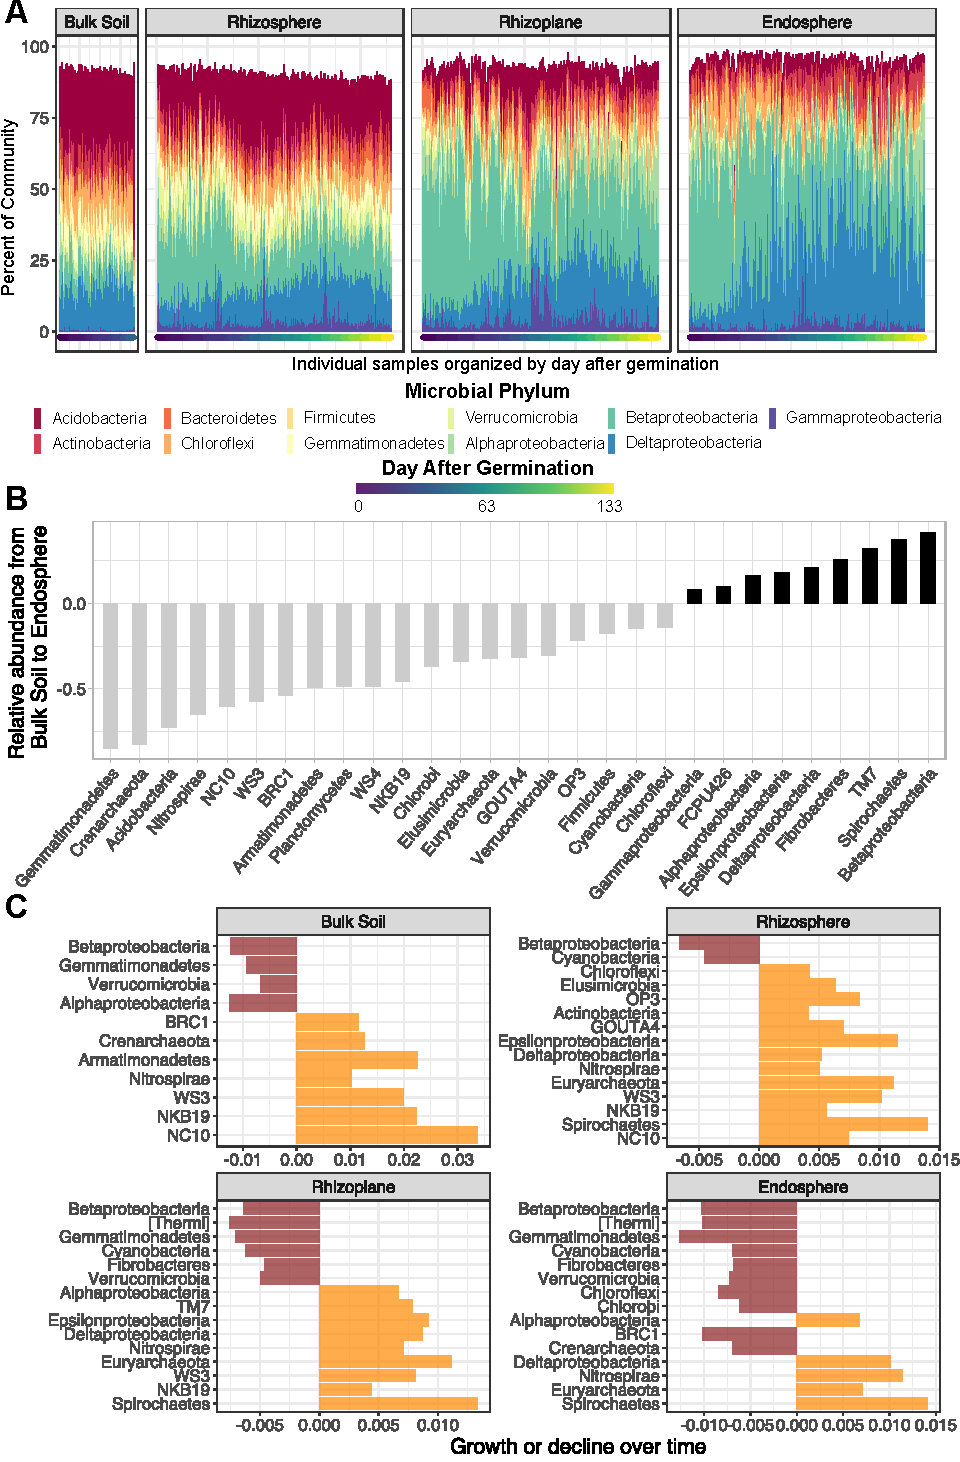
\includegraphics[width=4.25in]{Figures/figure3_2}
% where an .eps filename suffix will be assumed under latex,
% and a .pdf suffix will be assumed for pdflatex
\caption[Figure 4.2]{\textbf{Shifts in the microbiota over time are associated with increasing and decreasing phyla.} \textbf{(A)} Bar plots of the top 11 phyla abundance over the course of the seasons in each compartment. Each bar represents 1 sample that was taken throughout the course of the growing season. The bars are ordered by the age of the plant as indicated by the colored points beneath each bar. Both the 2014 and 2015 data were used for this graph. \textbf{(B)} Beta regression coefficient estimates for microbial phyla that are either increasing (above 0) or decreasing (below 0) in relative abundance from the outside of the root to the inside of the root. \textbf{(C)} Beta regression coefficient estimates for microbial phyla that are increasing (above 0) or decreasing (below 0) in relative abundance over the course of the seasons in each compartment.}
\label{Figure 4.2}
\end{figure}

We next sought to characterize the specific phyla responsible for the significant differences between the root-associated compartments and how these various phyla changed in abundance over the lifecycle of the rice plants. Figure 4.2A shows the relative abundance for the top 11 most abundant phyla between the compartments and how their abundance changes over the course of the season. Because the Proteobacteria phylum contains a broad phylogenetic makeup and because Proteobacteria make up the vast proportion of the rice root-associated microbiota, we further dissected the Proteobacteria phylum into its respective classes for this analysis. To model increasing or decreasing relative abundance of individual phyla between the various root-associated compartments, we assigned each compartment a value relative to its spatial position: bulk soil was position 1, rhizosphere was position 2, rhizoplane was position 3, and endosphere was position 4. We modelled how phyla either increased or decreased between these positions using beta regression. Beta regression is used for modeling dependent variables which lie in the interval (0, 1) and is thus useful for modelling individual taxa as a relative proportion of the total microbial community. 

Using this method, we were capable of identifying phyla which significantly differ in spatial distribution from the exterior to the interior of the root. Figure 4.2B indicates the degree of change for phyla whose relative abundance were significantly different across the root-associated compartments. The phyla are ranked in terms of how pronounced the changes are between the exterior and interior of the root. Those taxa which have values below zero on the y-axis are higher in relative abundance outside of the root, while taxa with a value greater than zero are higher in relative abundance inside of the root. Our analysis revealed more taxa with negative trends from the outside to the inside of the root which is consistent with the hypothesis that the root is a selective niche unsuitable for the growth of a large array of soil microbes. Many of the phyla found to be significantly enriched from the soil to the root interior belong to various classes within the Proteobacteria phylum. We found both Spirochaetes and Fibrobacteres to increase in abundance from the outside to the inside of the root. Both phyla are known to degrade cellulose, thus it is probable that these microbes are using the root tissue as an energy source or as a molecular cue for colonization \cite{Kudo1987,Ransom-Jones2012}.

We performed the same type of analysis to identify phyla that significantly increased or decreased in relative abundance over the course of the growing season in each compartment. Figure 4.2C shows the result of this analysis where we display the top 15 phyla in each compartment which show the highest degree of change over the course of the season. Below zero on the x-axis represents phyla that were reduced in relative abundance over the season, while vlaues above zero represents taxa that increased in abundance over the season. The plant associated compartments showed similarities in phylum increase or decrease over the season. For instance, in the rhizosphere, rhizoplane, and endosphere Betaproteobacteria consistently decreased over the course of the season, while Deltaproteobacteria, Euryarchaeota, and Spirochaetes all increased. These results indicate that the relatively large variances partitioned to differences in microbial communities across the root-associated compartments and over the course of the growing season can be explained by significant proportional shifts in various phyla.

\subsection{The composition of the root-associated microbiota is an accurate predictor of plant age}

\begin{figure}[h]
\centering
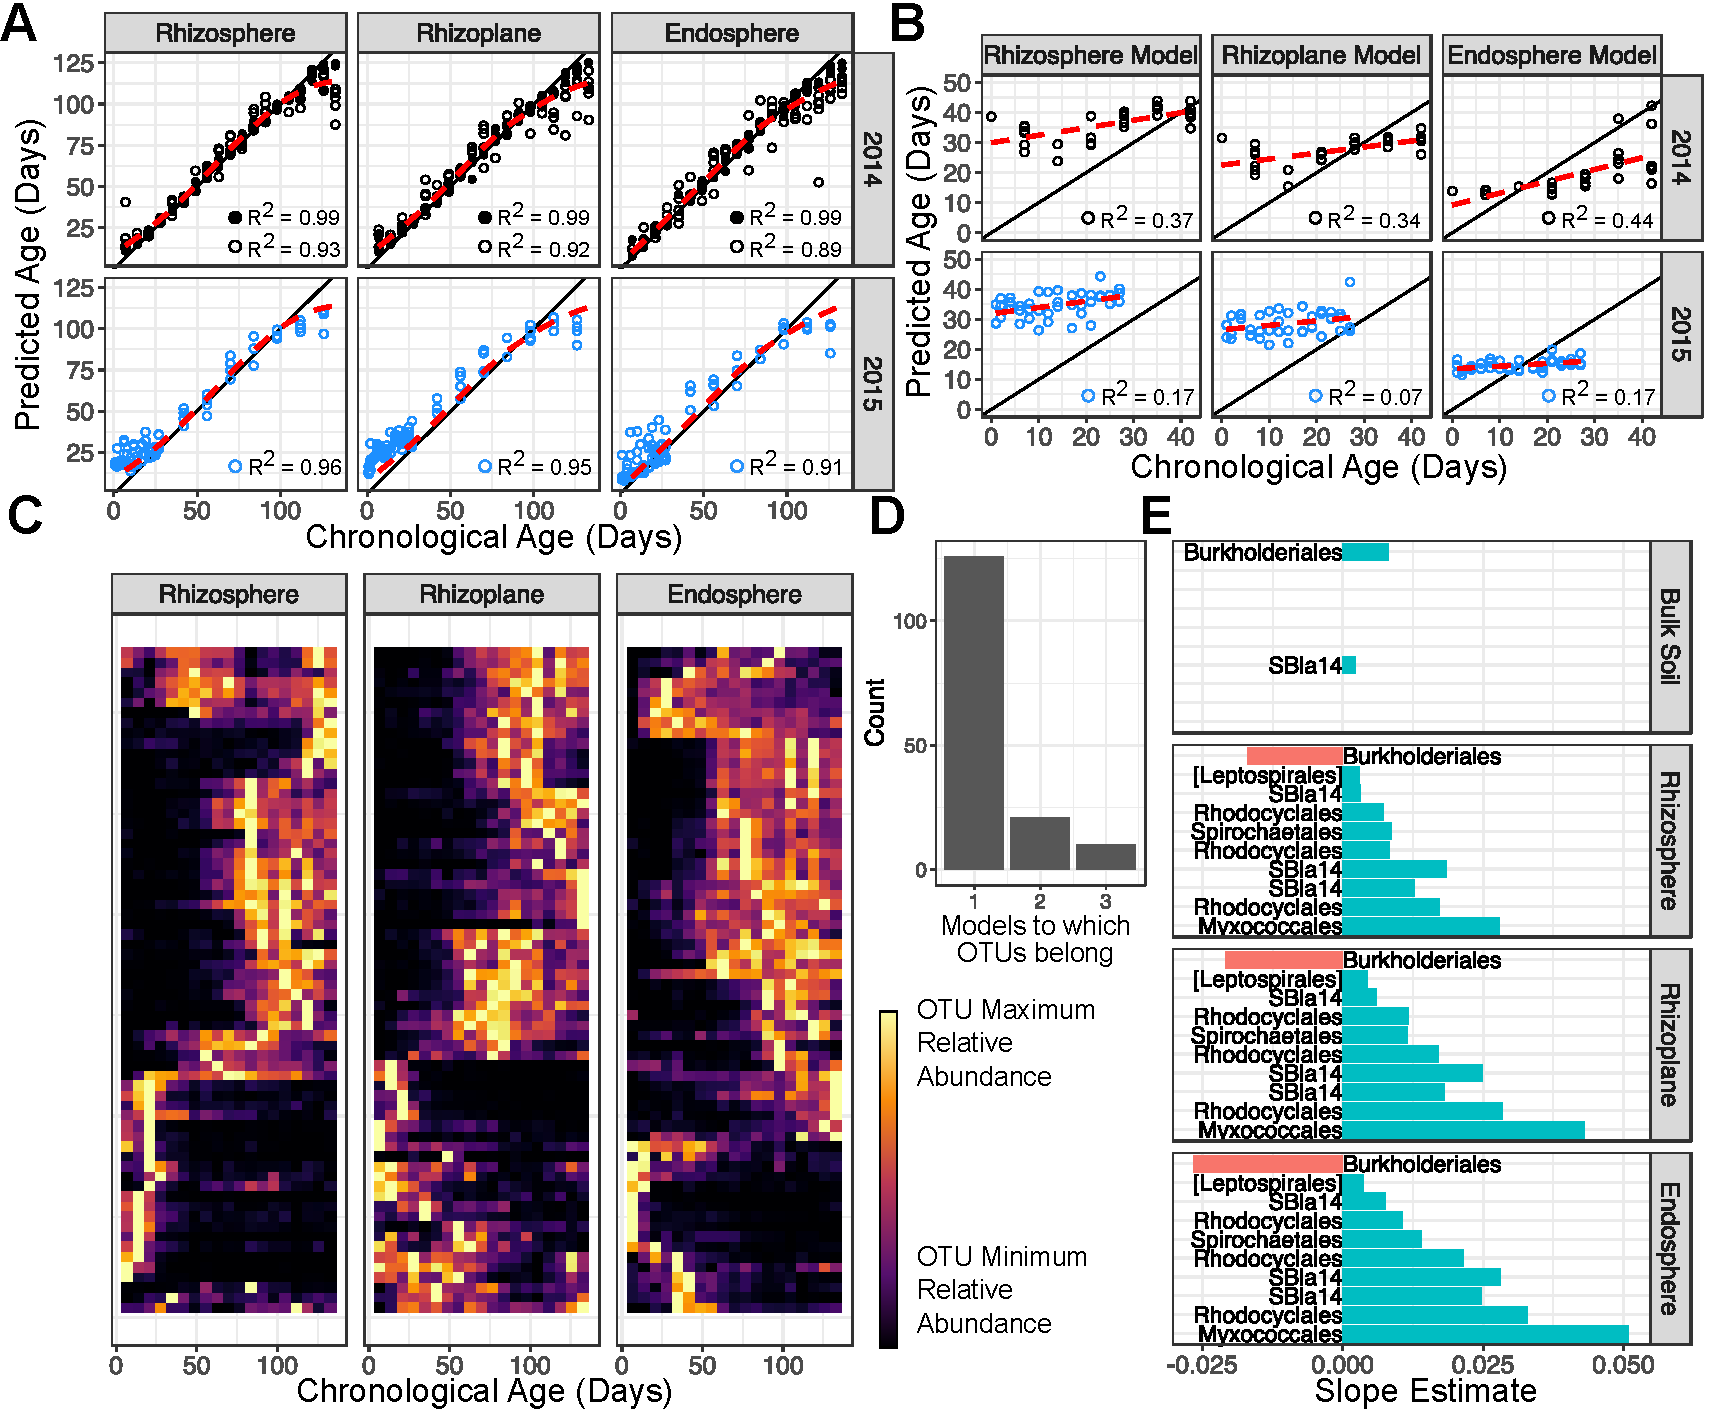
\includegraphics[width=6in]{Figures/figure3_3}
\caption[Figure 4.3]{\textbf{Figure 3. Random forests model detect taxa that are accurately predictive of plant age.} \textbf{(A)} The result of predicting plant age using the sparse RF models for the 2014 and 2015 season. Each point represents a predicted age value, solid points were the samples on which the models were trained and the hollow points are samples in which the model never encountered during training. The solid black line represents the perfect fit line (i.e. if a sample were to be perfectly predicted, it would fall on this line). The dashed red line is a Loess regression curve fit to the predicted data from the 2014 season to show how the predicted values deviate from the real values. Each Loess curve is specific to the respective compartment from the 2014 data. These same curves are plotted along with the 2015 data to show that the areas of deviation from the perfect fit line are similar in the 2015 data. \textbf{(B)} The values of the bulk soil samples as predicted by the compartment specific RF models. The dashed red line is a linear fit for the bulk soil samples in each compartment's model showing how the predictions deviate from the perfect prediction line. \textbf{(C)} A heatmap representing the abundance profiles of the 66 most age discriminant OTUs in each compartment over the course of the season. \textbf{(D)} The number of models the OTUs belong to. A value of 3 means that the particular OTU was shared in all three compartment specific models. \textbf{(E)} Shows the slope estimates of the 10 shared OTUs between the compartments to indicate whether the OTU is increasing or decreasing as a function of plant age. The Order of the OTUs are shown in text next to the bars.}
\label{Figure 4.3}
\end{figure}

Because there were notable patterns of microbiota shifts throughout the growing season in each root-associated compartment, we next sought to identify patterns in the abundance of various taxa to discriminate the age of the rice plants. This posed a formidable difficulty due to the underlying structure of our data and the biology of the microorganisms we are studying. In our dataset exist the abundance of many thousands of detectable microbes. The abundance pattern over time is unique for each detected microbe and some of these abundance patterns are useful for predicting the age of the rice plant while others have little to no utility for this purpose. Because of this problem, we settled on using the Random Forests (RF) algorithm, a machine learning technique, to model the age of the rice plants by using the abundance patterns of various microbes \cite{Breiman2001}. The RF algorithm is particularly suited for this task because it can incorporate multiple variables for consideration (i.e. using multiple OTUs for predictions), it does not assume linear trends in the input data nor does it require the data to have a parametric distribution, and it can return the importance values for the input features (i.e. it outputs how useful an OTU was for creating an accurate model). 

To begin, we regressed the abundances of all 8554 detected OTUs in a training set of samples from each root-associated compartment separately as a function of plant age to form the ``full'' RF models. Because various taxa had different abundance profiles over time between each compartment (Figure 2A), we surmised that each compartment should be modeled separately in order to make the most accurate prediction. The training data for each compartment is a random selection of four of the eight replicates within each time point from the 2014 season. The full models are not optimally accurate because some OTUs which are not useful for predictions can introduce a significant amount of error. We then conducted 10-fold cross validation on each model while subsequently removing non-important OTUs in order to identify how many of the most important OTUs should be included in each model (Fig. 4S1). This analysis revealed a marginal decrease in cross-validation error when using greater than 66 of the most important OTU features for each model. Thus, for each root-associated compartment, we formed a ``sparse'' RF model using the most important 66 OTUs derived from each compartment's full RF model. The sparse models were used for downstream analysis and were not subjected to any further parameter optimization.

We used the sparse models to predict the ages of plants from our test set of samples consisting of the remaining samples from the 2014 season which were not included in the training of the model. Each model predicted the new data accurately (Fig. 4.3A), with the lowest adjusted R2 value being 0.89 in the test set of the 2014 endosphere data. The least accurate timeframe for each model was after 100 days where each model consistently under-predicted the plants' ages, perhaps due to the overall stability of the root associated microbiome during the reproductive phase. We also predicted the ages of plants from the 2015 season using these sparse model. Again, we found the models to be accurate in their predictions of plant ages based off of the 66 OTUs included in each model. We used the sparse models to predict the ages of bulk soil samples for the 2014 and 2014 seasons (Fig. 4.3B). Each model consistently mis-predicted the age of the bulk soil samples. These results suggest that the 66 age discriminatory OTUs included in each model fluctuate over the growing season, i.e. some OTUs have increasing abundance over the season while other have decreasing patterns (Fig. 4.3C), and these patterns of fluctuations are consistent across different seasons. Furthermore, the 66 OTUs in each model are specifically predictive for the root-associated compartments and not for bulk soil samples, suggesting that the fluctuations in abundance for the sets of 66 OTUs are driven by the host plants and are not directly influenced by edaphic factors.

We next examined the top age discriminatory OTUs in each sparse model. The models consisted of phylogenetically diverse sets of taxa (Fig. 4S2): included in the models were OTUs from 14 Phyla, 33 Classes, 55 Orders, and 58 Families. Interestingly there was minimal overlap in OTUs between the models: we found only 10 OTUs to be conserved between all three models, while 126 OTUs were unique to a model (Fig. 4.3D). Of the ten overlapping OTUs, only one had a significantly decreasing abundance over the season in each root-associated compartment while the remaining nine had significantly increasing abundance patterns over the season in each compartment (Fig. 4.3E). Only two of these OTUs were found to also have either a significant increasing or decreasing trend in the bulk soil samples. Taxonomically, 7 of the 10 OTUs belong to the Betaproteobacteria class, specifically within the orders of SBIa14 and Rhodocyclales. Taken together, these data indicate while a small set of OTUs are shared between the models, the models use a broad phylogenetic diversity of OTUs to discriminate plant age.

\begin{figure}[h]
\centering
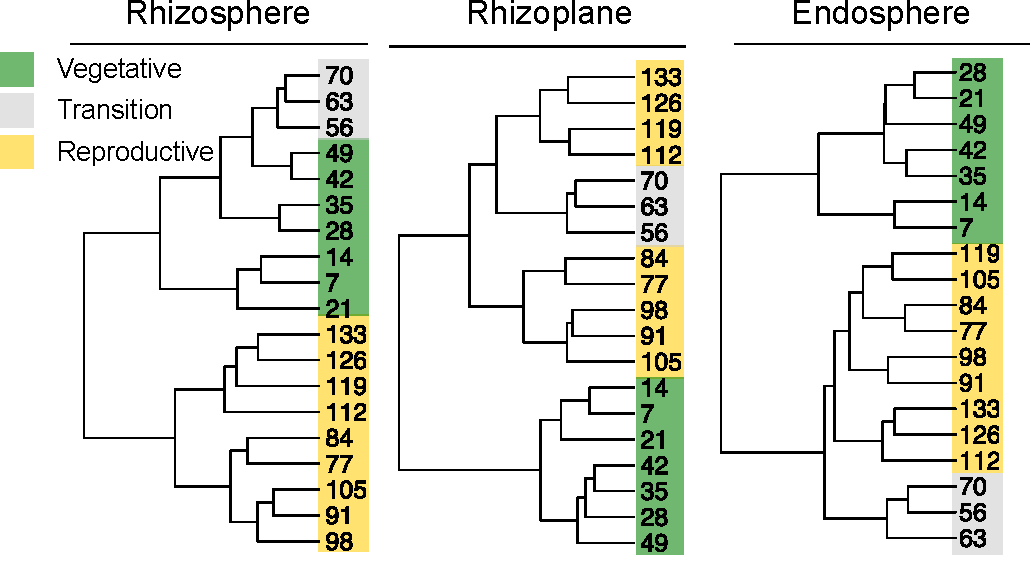
\includegraphics[width=5in]{Figures/rf_trees}
% where an .eps filename suffix will be assumed under latex,
% and a .pdf suffix will be assumed for pdflatex
\caption[Figure 4.4]{\textbf{Hierarchical clustering of time points based upon abundance of the 66 most age discriminant OTUs in each compartment's sparse RF model.} Colors represent the developmental stage that the plants were in when sampled. The numbers represent that host plant's age at the time of sampling.}
\label{Figure 4.4}
\end{figure}

We were next interested in understanding how the various time points relate to each other in terms of microbial community structure. That is, do time points cluster based upon developmental stages? To address this question, we performed hierarchical clustering using the 66 most age-discriminant taxa in each compartment (Fig. 4.4). The particular variety that was included in this study, M206, starts transitioning to the reproductive phase around 56 to 63 weeks after germination. In each compartment we found clear clustering of the time points during the vegetative phase. Consistently across each compartment, we found that the samples taken on day 56 through 70 cluster together. This is a transition time for the rice plants where they are switching from vegetative to reproductive growth. Interestingly, this transitory cluster falls closer to the reproductive or vegetative time points depending on the observed compartment. For instance, in the rhizosphere the transitory time points cluster with the vegetative samples and in the endosphere and rhizoplane the transitory time points cluster with the reproductive time points. This may suggest that the endosphere and rhizoplane microbiomes are the first to be affected by the transition to reproduction while the rhizosphere follows suit later.	

\subsection{Developmental stage is a driver of microbiota succession}
\begin{figure}[tbh]
\centering
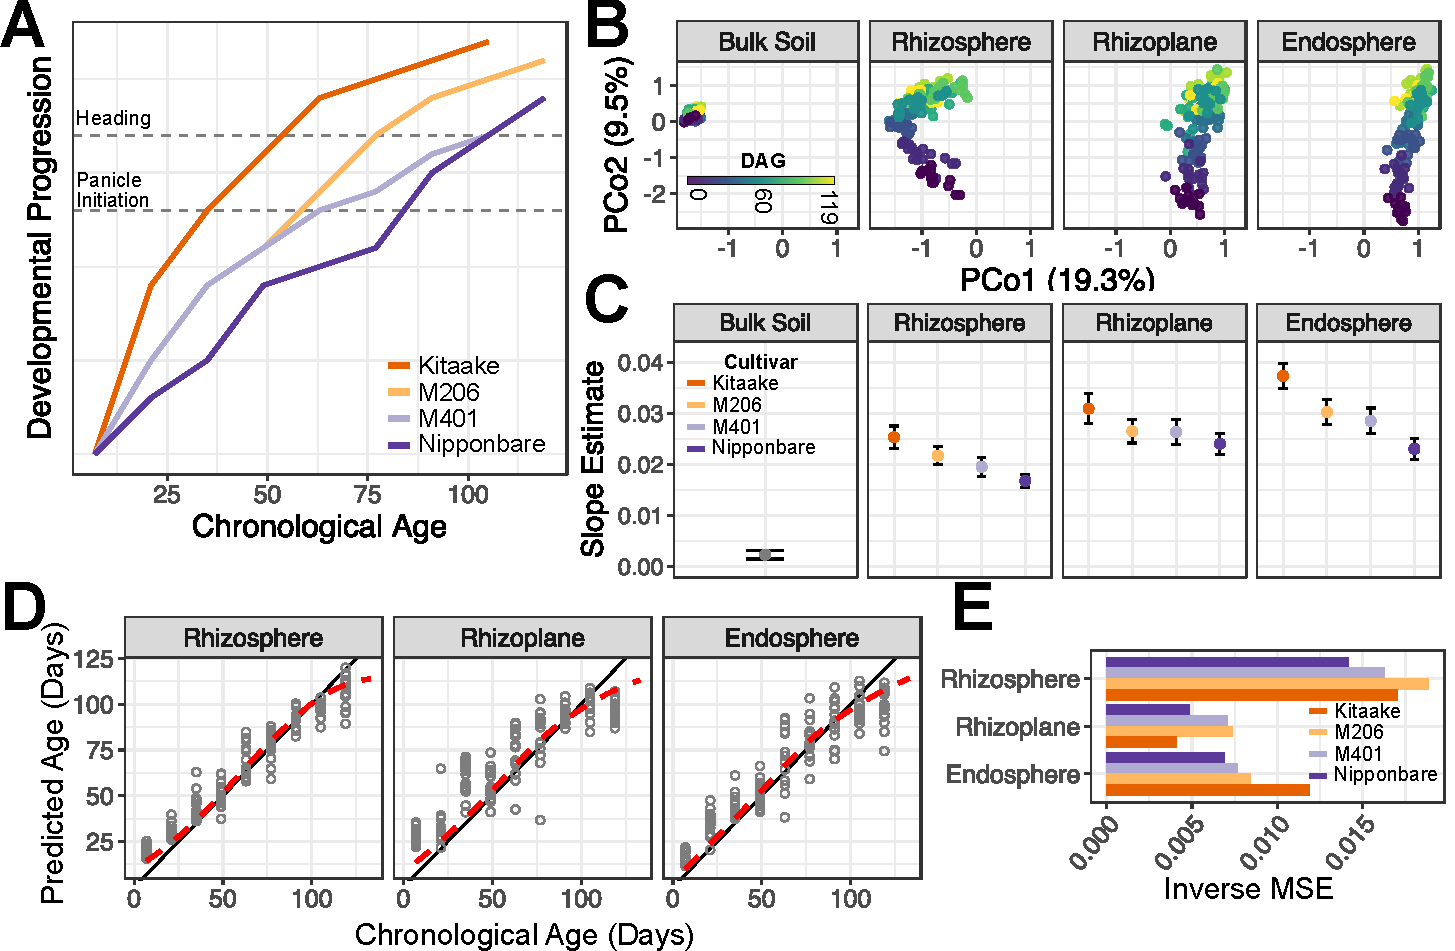
\includegraphics[width=6in]{Figures/figure3_5}
% where an .eps filename suffix will be assumed under latex,
% and a .pdf suffix will be assumed for pdflatex
\caption[Figure 4.5]{\textbf{Varieties with different developmental rates have different microbiota progressions.} \textbf{(A)} The developmental stage of the tested varieties as a function of plant age. We devised a numerical system for developmental progress based up morphological features indicative of developmental stage. \textbf{(B)} PCoA of the 2016 data indicating root-associated compartment and plant age are major determinants of microbiota structure. \textbf{(C)} Linear slope estimates for the principal coordinate 2 in panel B as a function of plant age for each variety and each compartment. A higher slope indicates that the microbiota is progressing faster along PCo2 as a function of plant age. \textbf{(D)} The predicted age of the 2016 data as predicted by the age discriminant sparse RF models. The solid black line is the perfect fit and the red dashed lines are the Loess curves calculated in Fig. 4.3A. \textbf{(E)} The inverse of the mean squared residual errors from panel D. A larger value means the model had more accurate predictions for the respective set of samples.}
\label{Figure 4.5}
\end{figure}

Our sparse models appear to be detecting shifts in the root-associated microbiota that correlate with developmental shifts in the rice plants. However, shifts in plant development also co-vary with shifting climatic and edaphic factors which may have indirect effects on the microbiota through various plant responses, thus making these factors difficult to uncouple from the effect of plant developmental stage on the shifting root-associated microbiota. Because our study was confined to one commercial field, we were limited to studying the dynamics of one rice variety throughout the 2014 and 2015 seasons which was synced in its developmental progression. To have a better idea of whether plant developmental stage significantly impacts the root-associated microbiota, we needed to un-sync plant age from developmental progression. In order to achieve this goal, we decided to grow rice varieties with different developmental rates in the same field in Arbuckle, CA. Plant genotype, while significant, has a relatively small effect on the root-associated microbiota compared to other environmental effects (such as drought), thus we chose 4 varieties from the tropical \textit{Japonica} sub-species of \textit{Oryza sativa} for this study, all with different developmental progression rates (Figure 5A). Kitaake, a variety often used by research labs because of its relatively fast generation to generation time, reaches the flowering stage faster than the rest of the included varieties. We included the California varieties M206 and M401 into this study. M206 is the variety that we have previously been studying in the Arbuckle field and the variety for which the sparse RF models were generated. Although M401 and M206 reach the panicle initiation stage around the same time, M401 has a much later heading data. We also included the variety Nipponbare, which reaches panicle initiation later than the rest of the varieties, but flowers within the same timeframe as M401. These varieties were water seeded in the Arbuckle field in a complete randomized block design (Figure 5A). We sampled plants within each plot every two weeks throughout the season, collecting rhizosphere, rhizoplane, and endosphere fractions from the plant roots. Our field design allowed us to also collect bulk soil samples throughout the entirety of the season as compared to the 2014 and 2015 seasons, which restricted our soil sampling due to the invasiveness of the rice roots. 

The data from the 2016 season had similar trends as exhibited in the 2014 and 2015 seasons. The root-associated compartments hosted distinct microbiotas (Fig. 4.5B, R2 = 0.27, P < 0.001) and the microbiota varied significantly due to plant age (Fig. 4.5B, R2 = 0.17, P < 0.001). We found that genotype had a very small overall effect on the root-associated microbiota (R2 = 0.01, P < 0.001). This level of variance is smaller than what we have previously detected in rice \cite{Edwards2015}. In our previous study, we grew 6 different cultivars in the greenhouse: 2 temperate \textit{Japonica}, 2 \textit{Indica}, and 2 \textit{Oryza glaberrima}. Our current study only used varieties within the temperate \textit{Japonica} clade, thus we expect that the reduced genetic diversity within this experimental population led to lower levels of microbiota variation compared out the previous study. We noticed that there was a significant statistical interaction between plant age and genotype (R2 = 0.05, P < 0.001), suggesting that the trends in microbiota shifts over the season differ depending on the rice genotype. To further inspect this observation, we calculated the slope of the second principal coordinate of Fig 5B as a function of plant age. We used the second principal coordinate because it was the axis best differentiating between plant age. We hypothesized that if plant developmental rate were to have an effect on the root associated microbiota, then the faster developing varieties would have steeper slopes than the slower developing varieties. Indeed, we found that Kitaake had the steepest slope in each compartment, while M206 and M401 have similar slopes and Nipponbare had the most gradual slope in each compartment. Bulk soil, however, had a much reduced slope over the season and is almost flat. Taken together these results indicate that microbiota shifts throughout the season are directly driven by the host plant and the rate of these shifts correlate with the developmental progression rate of the host plant.

\subsection{Developmental stage is a driver of microbiota succession}
\begin{figure}[tbh]
\centering
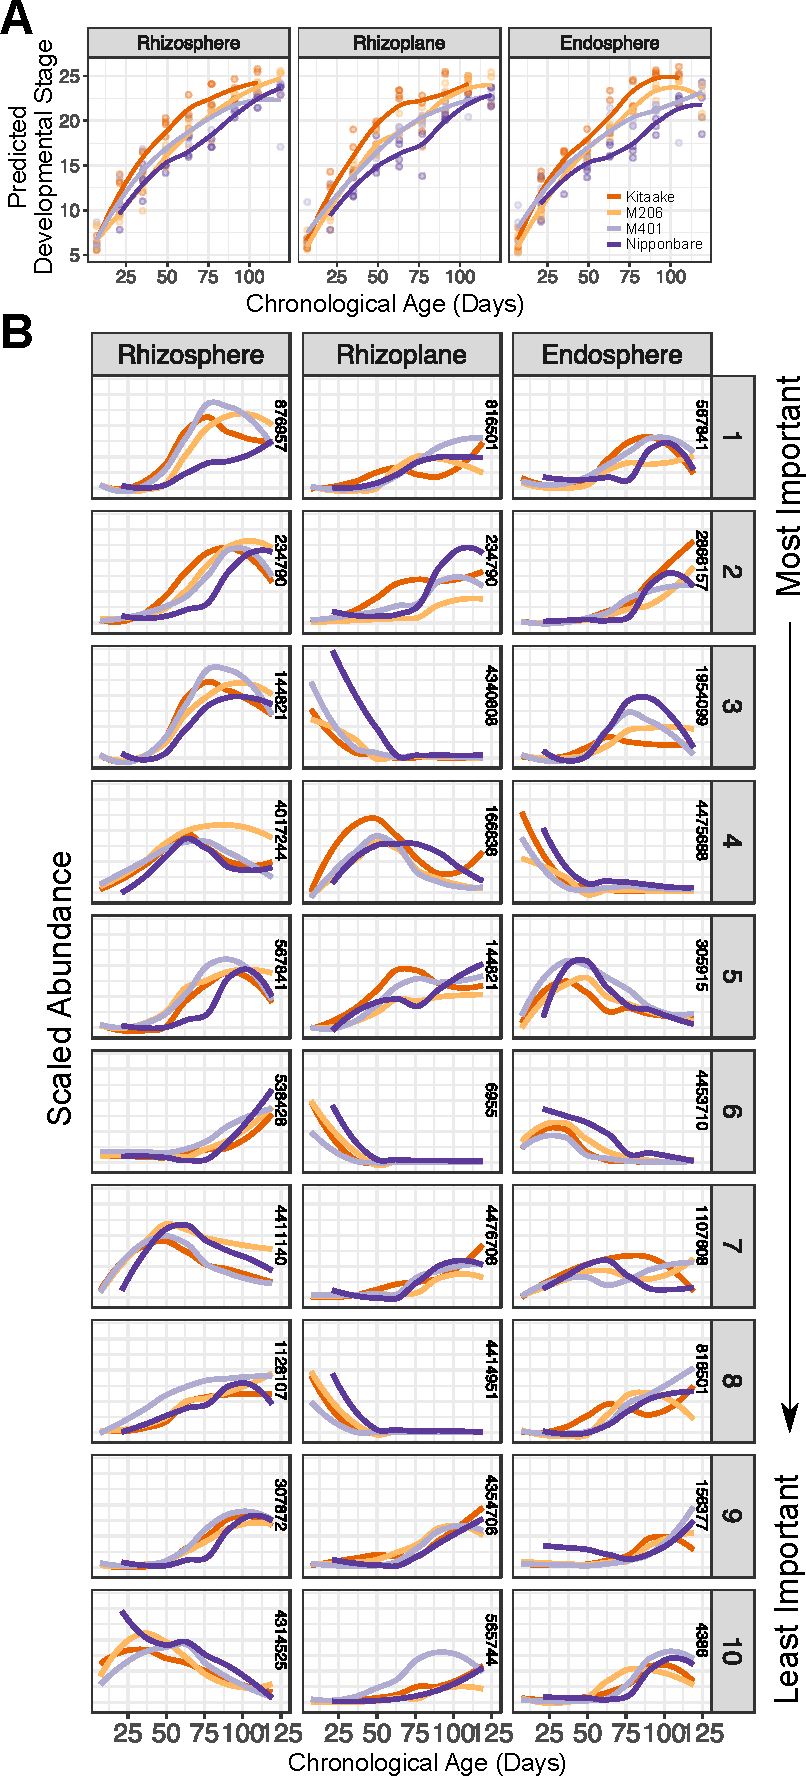
\includegraphics[width=3in]{Figures/figure3_6}
% where an .eps filename suffix will be assumed under latex,
% and a .pdf suffix will be assumed for pdflatex
\caption[Figure 4.6]{\textbf{Random forests model detect taxa that are accurately predictive of plant developmental stage.} \textbf{(A)} Results of the model after predicting developmental stages of the samples taken from the 2016 season in each compartment plotted as a function of plant age. The different varieties separate similar to the pattern exhibited in Figure 5A. \textbf{(B)} The abundance profiles of the top 10 most developmental stage discriminant taxa in each compartment over the course of the 2016 season.}
\label{Figure 4.6}
\end{figure}

We next used the sparse RF models to predict the age of samples taken from the 2016 season (Fig. 4.5D). The models were remarkably accurate at predicting the ages of plants from the 2016 season despite the differences in the developmental progression rates of the genotypes. We calculated the mean squared error (MSE) of residuals for each genotypes predicted values by the compartment specific sparse RF models (Fig. 4.5E). In the case of the rhizosphere and rhizoplane, the age of the M206 genotype was most accurately predicted by the models (it was the second most accurately predicted variety using the endosphere models). The original models were trained on data collected from M206 during the 2014 season. These results suggest that the accuracies of the models are affected by the differences between the genotypes likely due to variation in developmental progression rate. 

To have a better understanding of which microbes are associated with the various developmental stages, we formed new RF models for predicting plant developmental stage rather than plant age. Development in plants is a continuous process marked by numerous stage-specific morphological features. We monitored the developmental stage of the genotypes throughout the season assigning a numerical value from 1-27, with a value of 1 corresponding to a recently germinated seeding and 27 corresponding to a senescent plant. Panicle initiation corresponded to a value of 18, thus a plant that is transitioning to the reproductive phase has a value of 18 or higher and a plant in the vegetative phase has a value of 17 or lower. We followed the same approach as previously mentioned to develop the RF models. Briefly, we trained full RF models in each compartment where we regressed the full dataset of OTUs against the developmental stage number for a training set of samples. From these full models, we sequentially removed OTUs of lower importance while performing 10-fold cross validation. We found that the models were near peak accuracy when including 29 of the most important OTUs for each compartment (Fig. 4S3). With these 29 most-important OTUs, we developed sparse RF models that modelled the microbiota as a function of plant developmental stage. When the predicted values of plant developmental stage were plotted as a function of the plant's chronological age, we found that the predictions accurately matched the developmental progressions that we witnessed in the field (compare the prediction plot in Fig. 4.6A to the plot of witnessed developmental progressions in Fig. 4.5A). These results indicate that the sparse RF models were able to detect shifts in the microbiota that correlate with developmental shifts in the plant. The abundance profiles for each the top 10 most important OTUs for each compartment's model's accuracy are plotted in Fig. 4.6B. The developmental stage sparse RF models used less OTUs than the plant age models to make accurate predictions. This suggests that the total root-associated microbiome is more affected by the chronological age of the plant rather than the plant's developmental stage.

\section{Discussion}
Annual plants quickly undergo large shifts in morphology and physiology throughout their lifecycle \cite{Freeling1990,Moldenhauer}. Developmental shifts are accompanied by different nutritional requirements and source sink relationships \cite{Ishimaru2013,Tegeder2010} which in turn could affect the compositional profile of the root-associated microbiota. Here we have detailed how the root-associated microbiota shift throughout the life cycle of rice plants growing in a single field in Arbuckle, CA. We found that the microbiota shifts significantly over time, with most of these shifts happening in the vegetative phase of developmental and a stabilization of the microbiota occurs after the entry into the reproductive phase. We found that there are large shifts in various phyla throughout the season. Members of the Deltaproteobacteria class predominantly increased over the season and members of the class Betaproteobacteria predominantly decreased over the season. We found that these patterns held over multiple seasons and that seasonal effects were of minimal importance on the overall root-associated microbiota. The bulk soil community members are relatively stable compared to the root-associated microbiota, suggesting that the plant non-randomly controls the fluctuating abundances of various taxa throughout the season. We found that the microbiota is predictive of plant age by fitting sparse random forests models to each compartment. These models identified many plant age discriminant microbial taxa which reproducibly changed in abundance over the course of the season. The mechanisms by which plants control the structure of their root-associated microbiota is unknown. Using cultured representatives from these age-discriminant microbial taxa in controlled inoculation experiments could help elucidate these processes and may suggest various roles for members of the root-associated microbiota on host health. 

From our initial results, it remained unclear whether plant developmental stage was indeed a regulator of the root-associated microbiota structure. A recent study claimed that the entry into flowering likely has no effect on the root-associated microbiota \cite{Dombrowski2016}. The authors conducted a clever experiment by growing a very early flowering \textit{Arabis alpina} mutant, \textit{perpetual flowering1} (\textit{pep1})\cite{Wang2009}, along with wild type Arabis alpina. They collected samples from the rhizosphere and endosphere of each genotype after 6, 12, and 28 weeks of growth (the pep1 mutant flowers after 12 weeks). They found no significant differences in the microbiotas taken from the flowering mutant and the still vegetatively growing wild type plants. They did, however, find significant differences in root-associated microbiotas between the different time points. These results led the authors to conclude that the root-associated microbiota is affected by plant residence time (i.e. the chronological age of the host plant) but not the developmental stage. \textit{Arabis alpina} (a wild \textit{Arabidopsis thaliana} relative) is a perennial plant, and is thus physiologically distinct from rice plants. We tested the hypothesis ourselves of whether fluctuations in the microbiota are correlated with different developmental stages by growing several rice varieties with different flowering times under field conditions and sampling their root microbiota throughout the growing season. We found that the progression of the microbiota throughout the season is correlated with the developmental progression of the plant and that these progressions are not found in the microbiota of unplanted soil. We developed models to predict the developmental stages of the plants using the abundance of various members within the plants' root-associated microbiota. From these models we were able to extract various microbes whose abundance profiles are predictive of plant developmental stage. Isolating these candidate microbes in pure culture would allow for a deeper investigation of how host plants communicate with their microbiota during various developmental and physiological states.

The random forests models trained to discriminate plant age detected more microbes than the random forests models trained to predict plant development. This discrepancy is indicative that plant age has a larger impact on the overall structure of the root-associated microbiota than plant developmental stage, yet plant developmental stage is still an important factor for differentiating the root-associated microbiota. Our results are clearly different than the aforementioned study that found no microbes to be affected by plant developmental stage. There are several likely causes for this discrepancy. Arabis alpina is a wild perennial plant species and rice is a domesticated annual crop species. One hallmark trait of cereal domestication is the selection for varieties with larger sink sizes in the seed \cite{Ishimaru2013}. For instance, in wild grass species, source carbohydrates are more evenly distributed to various sink tissues in the plant than domesticated cereals, where the seeds are a predominant sink \cite{Shomura2008,Ishimaru2013}. The discrepancy between sink-source dynamics in these two host plants could, at least partially, explain why our study detected shifts in the microbiota due to developmental stage while it was undetected in Arabis. In rice, accumulation and storage of carbohydrates in the stems occur until the onset of reproduction, after which internal signals program the host plant to begin repartitioning carbohydrates to the developing panicle and to the filling grain \cite{Slewinski2012,Scofield2009}. These host signals, along with the shifting nutritional needs at this stage could explain the stabilization in the microbiota that occurs at the onset of reproduction. Here we have a provided one of the first links between host plant development and composition of the root-associated microbiota. Understanding the physiological, molecular, and developmental signals from the host plant that affect the root-associated microbiota may unlock the use of microbes to boost plant performance and yield.
	
\section{Materials and Methods}
%
\subsection{Plant growth and sampling during the 2014 and 2015 seasons}
%
We collected samples from a commercially cultivated rice field in Arbuckle, CA. In both seasons the field was water seeded in early May. Water seeding is conducted by first preparing the field by removing winter vegetation, disking the soil to produce baseball sized clods, applying nutrients, and then flooding \cite{Hardke}. The rice seeds are soaked in water overnight and then loaded into an aircraft where they are then applied aerially to the field in an even density. For this particular field, the farmer grew the M206 cultivar, a medium grained California variety that has an average heading date of 86 days after germination \cite{Linquist2012}. We began sampling plants 7 days after the fields were seeded, which coincided with the emergence of the seminal roots. In the 2015 and 2016 seasons we restricted our area of sampling to a 150 x 150 foot plot. Within this plot we would sample plants from random locations. Our sampling occurred as previously described. Using gloved hands, would scoop under the root mass to separate the plant from the ground. Grabbing the plant by the base of the stem, we would then shake the plant to remove loosely attached soil from the roots. We would then place the roots with tightly adhering soil into 50 mL Falcon tubes with 15 mL autoclaved phosphate buffered saline (PBS) solution. We would then bring the samples back to the laboratory at UC Davis. We collected bulk soil samples as the season allowed. During the later parts of the season it became impossible to find soil samples unaffected by rice roots.

\subsection{Plant growth during the 2016 Season}%
We grew various cultivars in the same field in Arbuckle, CA for the 2016 season. Briefly we designed a fully randomized block design to grow these varieties in 1 x 1 m plots in quadruplicate. We left 0.5 m wide walking lanes between each plot which subsequently allowed us to sample bulk soil throughout the course of the growing season. To be consistent with the previous years' methods, we water seeded these varieties. This entailed soaking the seeds in a 2\% bleach solution for 4 hours to remove the risk of the field being contaminated \textit{Fusarium moniliforme}, a seed borne fungal pathogen that causes the disease Bakanae. The seeds were then washed 3 times with sterile water and soaked overnight. We then hand seeded each plot at similar density as what the farmer had applied in previous seasons. At each timepoint the plants were sampled as previously described and transported to the lab for further processing. The plants used for sampling during this season were dissected to score various developmental stages between the cultivars \cite{Moldenhauer}.

\subsection{Separation of the root-associated compartments and DNA extraction}
%
The root associated compartments were separated as previously described \cite{Edwards2015}. The roots with soil attached were vortexed in PBS solution and 500 uL of the resulting slurry was used for DNA extraction. The roots were cyclically washed in fresh PBS solution until no soil particles were visible in the solution. The roots were then placed into fresh PBS and sonicated for 30 s to remove surface cell layer of the roots. The resulting slurry was centrifuged down to concentrate the biomass and then used as the rhizoplane fraction for DNA extraction. The remaining roots were sonicated twice more, refreshing the PBS solution at each stage, and then ground in the bead beater. The resulting solution was used for DNA extraction as the endosphere fraction. All DNA extraction was performed using the MoBio Powersoil DNA isolation kits.

\subsection{PCR amplification and sequencing}
%
We amplified the V4 region of the 16S ribosomal RNA gene using the universal 515F and 806R PCR primers. Both our forward and reverse primers contained 12 base pair barcodes, thus allowing us to multiplex our sequencing libraries at well over 150 libraries per sequencing run. Each library was accompanied by a negative PCR control to ensure that the reagents were free of contaminant DNA. We purified the PCR products using AMPure beads to remove unused PCR reagents and resulting primer dimers. After purification, we quantified the concentration of our libraries using a Qubit machine. Our libraries were then pooled into equal concentrations into a single library and concentrated using AMPure beads. The pooled library then went through a final gel purification to remove any remaining unwanted PCR products. Pooled libraries were sequenced using the Illumina MiSeq machine with 250 x 250 paired end chemistry. 

\subsection{Sequence Processing, OTU clustering, and OTU filtering}
%
The resulting sequences were demultiplexed using the barcode sequences by custom Python scripts. The sequences were quality filtered and then assembled into full contigs using the PandaSeq software \cite{Masella2012}. Any sequences containing ambiguous bases or having a length of over 275 were discarded from the analysis. The high-quality sequences were clustered into operational taxonomic units (OTUs) using the Ninja-OPS pipeline \cite{Al-Ghalith2016} against the Green Genes database \cite{DeSantis2006} and then assembled into an OTU table. This OTU table was filtered to remove plastidial and mitochondrial OTUs and filtered to remove OTUs that occur in less than 5\% of the samples. This process removed the total OTU count from 24,048 to 8,554 taxa. The resulting 8,554 taxa were used for the analysis.

\subsection{Statistical Analysis}
%
All statistical analyses were conducted using R version 3.1 \cite{RCoreTeam2016}. Unless otherwise noted, we determined statistical significance at $\alpha$ = 0.05 and, where appropriate, corrected for multiple hypothesis testing using the false discovery rate method. Shannon diversity was calculated using the diversity() function, PCoA analyses were conducted using the capscale() function, perMANOVA was conducted using the adonis() function, and community structure variability was measured using the betadisper() function all from the Vegan package \cite{Oksanen2013}. Linear models were run using the lm() function and ANOVA was run using the aov() function. Beta regression was used to model proportion of any given phylum ($\mu_p$) as function of distance from the root ($x_2$) using the betareg() function from the BetaReg package \cite{Cribari-Neto}. To do this, we assigned each compartment a value from the outside to the inside of the root: bulk soil had a value of 1 and endopshere had a value of 4. The model is described by the equation
\begin{equation}
    g(\mu_p) = \beta_1 + \beta_2 x_{p2}
 \end{equation}
 We also used beta regression to model trends in proportions for a given phylum ($p$) in a given compartment ($c$) as a function of host plant age ($x_2$) using the equation
 \begin{equation}
 	g(\mu_{pc}) = \beta_1 + \beta_2 x_{pc2}
 \end{equation}
 For each model, we used a logit link function. Random forests models were generated and analyzed using the randomForest package \cite{Liaw2015}. All graphs and plots were generated using the ggplot2 package \cite{Wickham2009}. R notebooks for the full analyses can be found on GitHub (https://github.com/bulksoil).

\newpage

\begin{figure}[h]
\centering
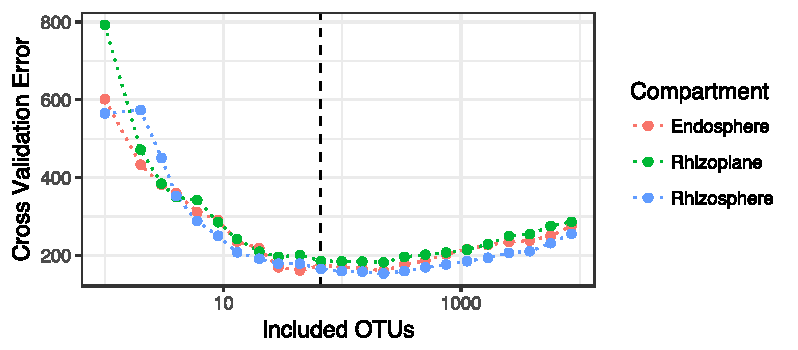
\includegraphics[width=5in]{Figures/figure3_s1}
\captionsetup{labelformat=empty}
\caption[Figure 4S1]{\textbf{Figure 4S1. Cross validation error of models predicting plant age while sequentially removing less important OTUs for model accuracy.} This analysis revealed that 66 of the most important OTUs should be included for the models to be the most accurate for predicting plant age.}
\label{Figure 4S1}
\end{figure}

\newpage

\begin{figure}[h]
\centering
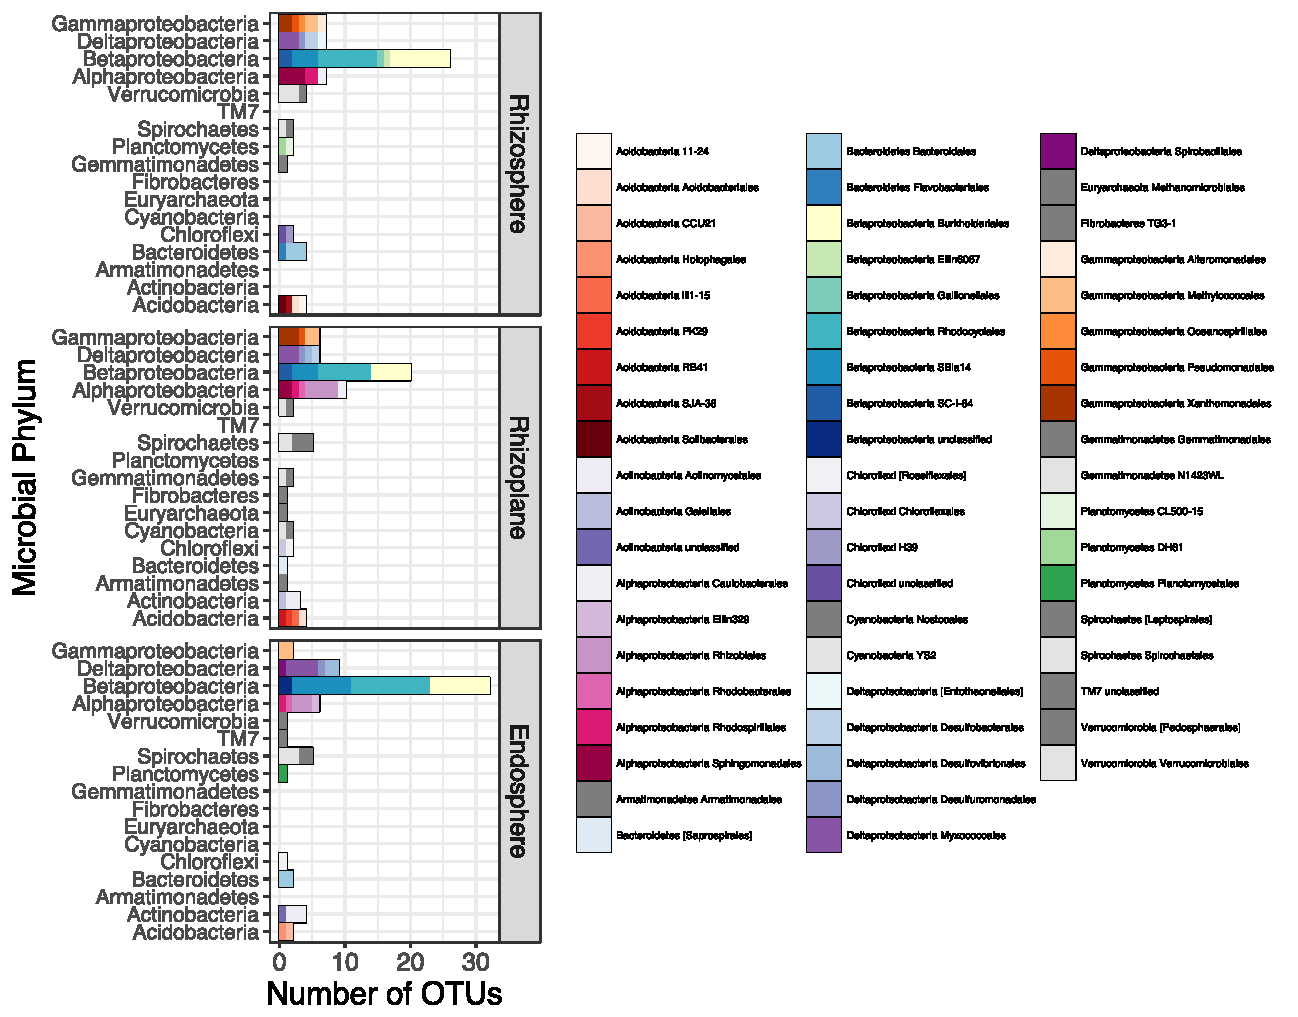
\includegraphics[width=6in]{Figures/figure3_s2}
\captionsetup{labelformat=empty}
\caption[Figure 4S2]{\textbf{Figure 4S2. The orders of the 66 most important OTUs used in the sparse RF models predicting plant age.}}
\label{Figure 4S2}
\end{figure}

\newpage

\begin{figure}[h]
\centering
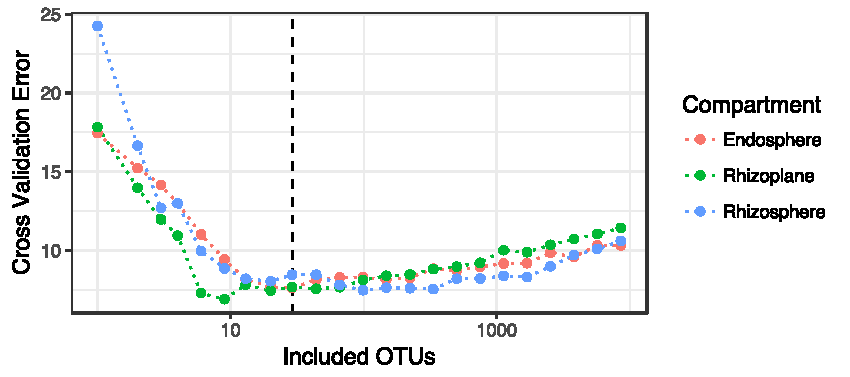
\includegraphics[width=4in]{Figures/figure3_s3}
\captionsetup{labelformat=empty}
\caption[Figure 4S3]{\textbf{Figure 4S3. Cross validation error of RF models predicting plant developmental stage while sequentially removing less important OTUs for model accuracy.} This analysis revealed that 29 of the most important OTUs should be included for the models to be the most accurate for predicting plant age.}
\label{Figure 4S3}
\end{figure}